

\documentclass{article}
\usepackage[utf8]{inputenc}
\usepackage[english]{babel}
\usepackage[]{amsthm} %lets us use \begin{proof}
\usepackage[]{amssymb} %gives us the character \varnothing
\usepackage{graphicx}
\usepackage{hyperref}
\usepackage{multicol}


\title{Homework 1}
\author{Aasim Zahoor}
\date\today


\begin{document}
\maketitle 


\begin{center}
\section{Problems}
\end{center}
\textbf{Link}\vspace{1.5em}
\url{https://github.com/AasimZahoor/Comp_methods.git}
\vspace{1.5em}

\textbf{Problem 1}\vspace{1.5em}

In the code for Problem 1 I have defined five functions. They are:
\begin{itemize}
\item{\textbf{midpoint(f,a,b,n)}}\item{\textbf{trapezoid(f,a,b,n)}}\item{\textbf{simpson(f,a,b,n)}}\vspace{0.2em}

These functions have the same arguments and thet are f= 'the function being integrated', $[a,b]$='The range of integration', n='The number of steps'. All of them need to be inputted while calling the function.
\vspace{0.2em}

\item{\textbf{diff(f,a,h=0.000001)}}\vspace{0.2em}

This function differentiates the function f at point a. h represents the step size and has a default value of $0.000001$\vspace{0.2em}

\item{\textbf{g()}}\vspace{0.2em}

This is a test function and can be used to test these function. You would need to make changes in the code to test different function.
\vspace{0.2em}
\end{itemize}

\emph{\small{Testing the functions using sine function(the figure on the left), the results of the test(the figure on the right)}}
\begin{center}
\begin{multicols}{2}
	\begin{center}
        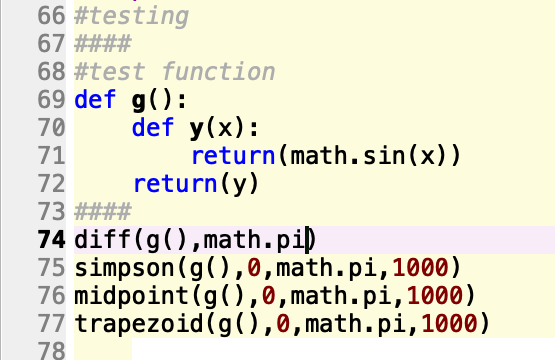
\includegraphics[scale=0.5]{Images/pb1test}
        \end{center}
\columnbreak
       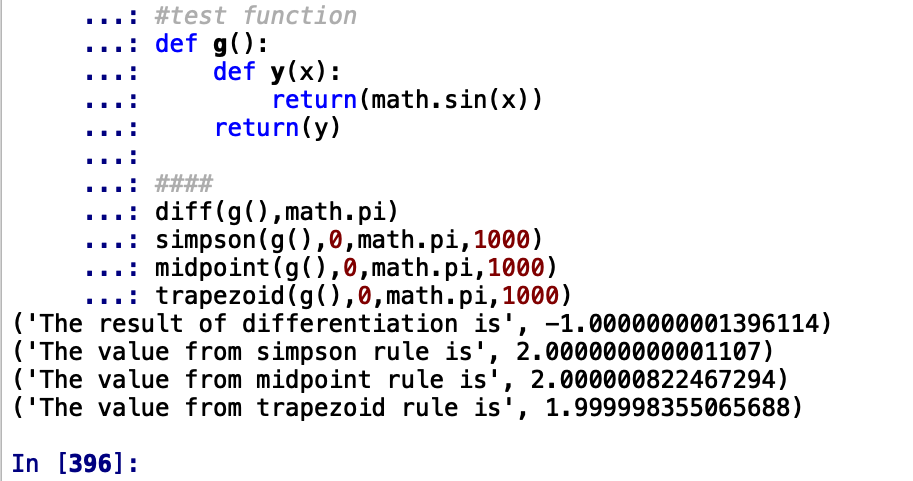
\includegraphics[scale=0.37]{Images/pb1testp}
\end{multicols}
\end{center}
\vspace{0.2em}






\vspace{1.5em}
\textbf{Problem 2}\vspace{1.5em}

The problem asked us to do four things for a given value of c and V200. In my code(which hopefully has enough comments that it is easier to understand) I have defined three functions, two to give the Mass enclosed as output (one function gives a value of mass enclosed at r and one gives a function in terms of r, which I used to test my approximation I used  in finding the mass in a shell) and one to give Vc. I calculated the mass enclosed in a halo by taking r=300kpc, the mass in a little shell was also found at r=300kpc with a thickness of 1 kpc. I also calculated the derivative at r=300kpc and has a h =0.00001kiloparsec (small increment which we use in the definition). Then I changed V200 values [60,160,260,360] while keeping c=15. Then I changed c values [5,15,25,35] while keeping V200=160km/s. From the figure it appears the curve flattens which is expected as the density decreases as we move away and hence the mass becomes constant. Also, the product of differentiation at r=300kpc is negative showing that mass of shells is decreasing at that point , making the previous observation more solid.
\vspace{0.2em}

I calculated mass of the shell using midpoint too and it agrees reasonably well with my approximation. 

\begin{center}
\begin{multicols}{2}
	\begin{center}
        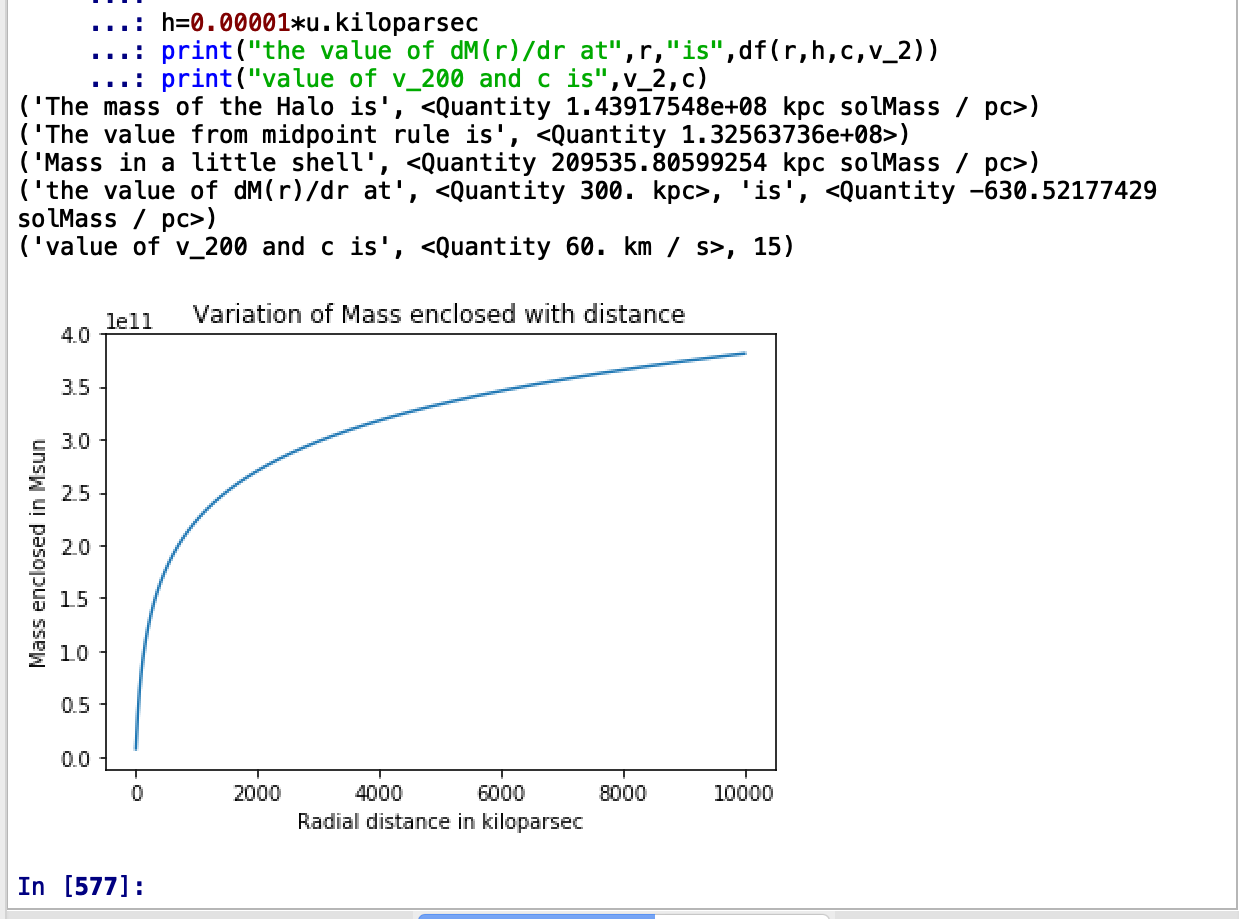
\includegraphics[scale=0.25]{Images/60}
        \end{center}
\columnbreak
	\begin{center}
       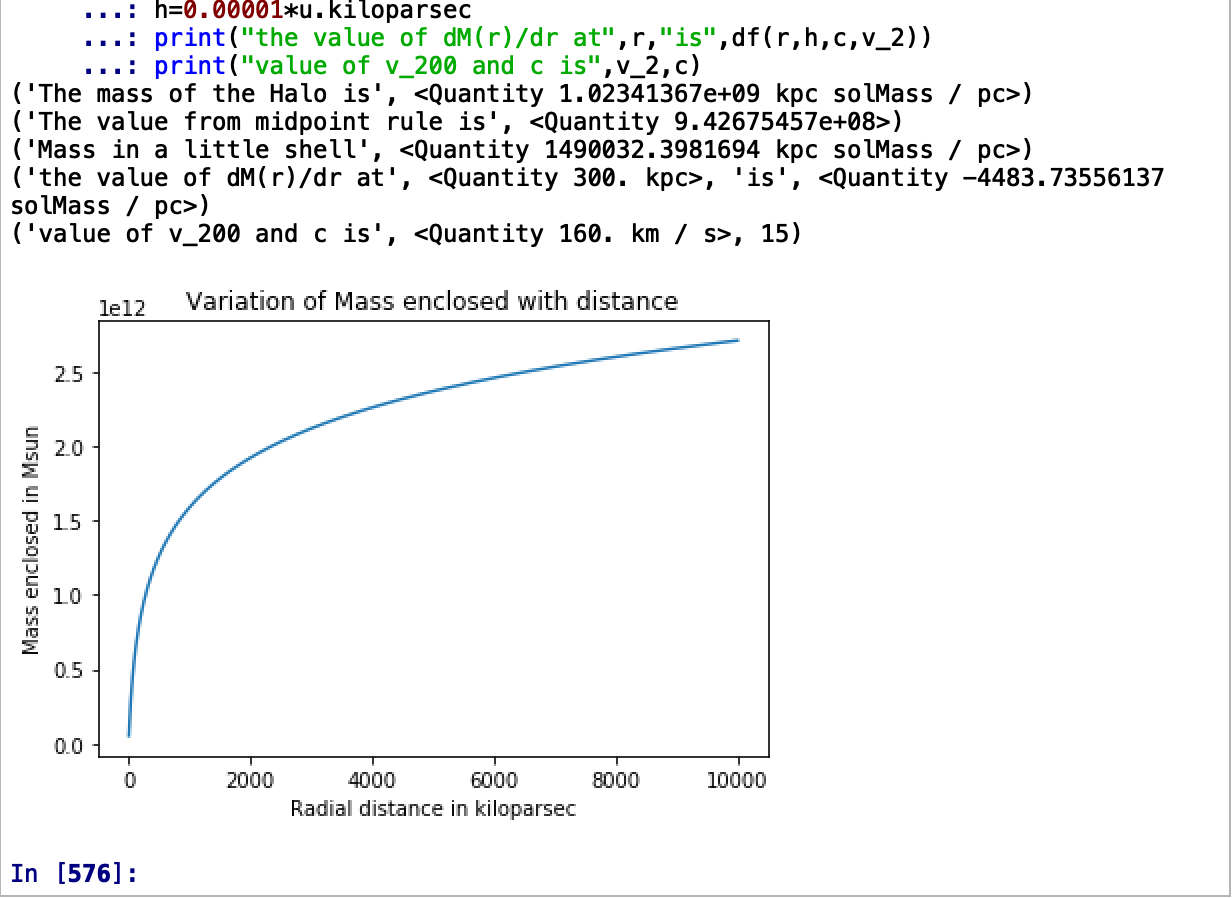
\includegraphics[scale=0.25]{Images/160}
       \end{center}
\end{multicols}
\end{center}

\begin{center}
\begin{multicols}{2}
	\begin{center}
        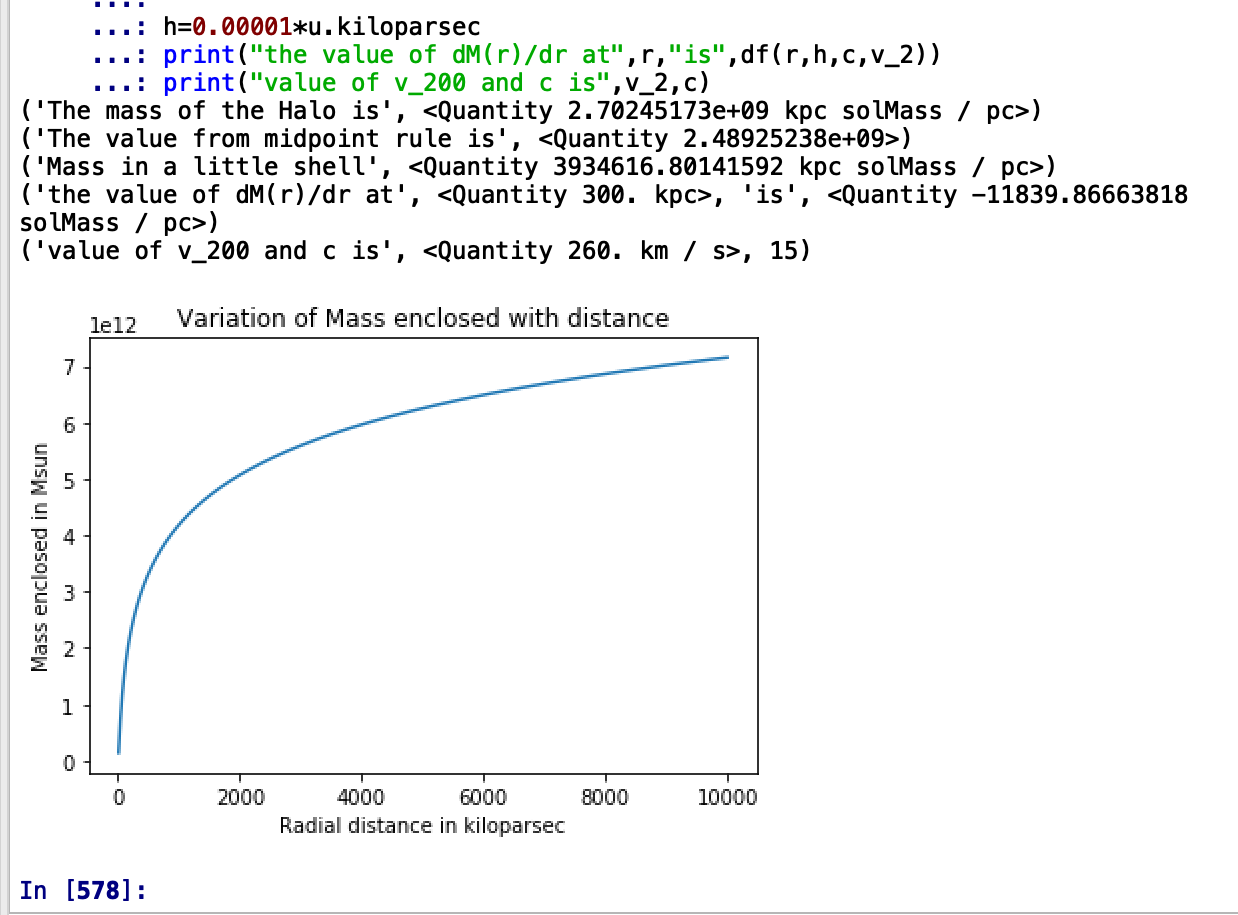
\includegraphics[scale=0.25]{Images/260}
        \end{center}
\columnbreak
	\begin{center}
       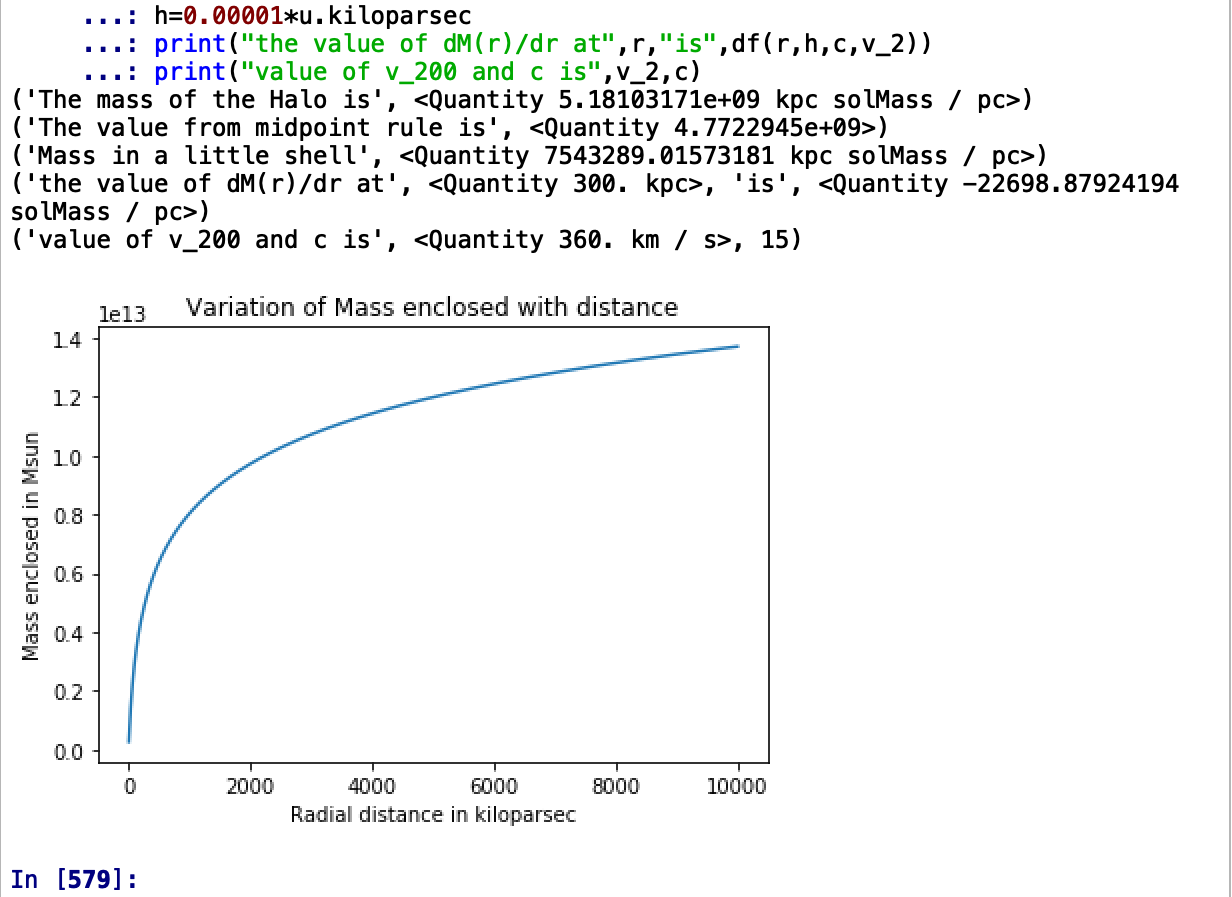
\includegraphics[scale=0.25]{Images/360}
       \end{center}
\end{multicols}
\end{center}


\emph{\small{These figures show output when I kept c fixed to 15 and changed V200.}}

\vspace{0.2em}

As I increased V200 while keeping c constant, value of mass in a halo, mass in the shell increased but the dM(r)/dr became more negative.
 
 
 \begin{center}
\begin{multicols}{2}
	\begin{center}
        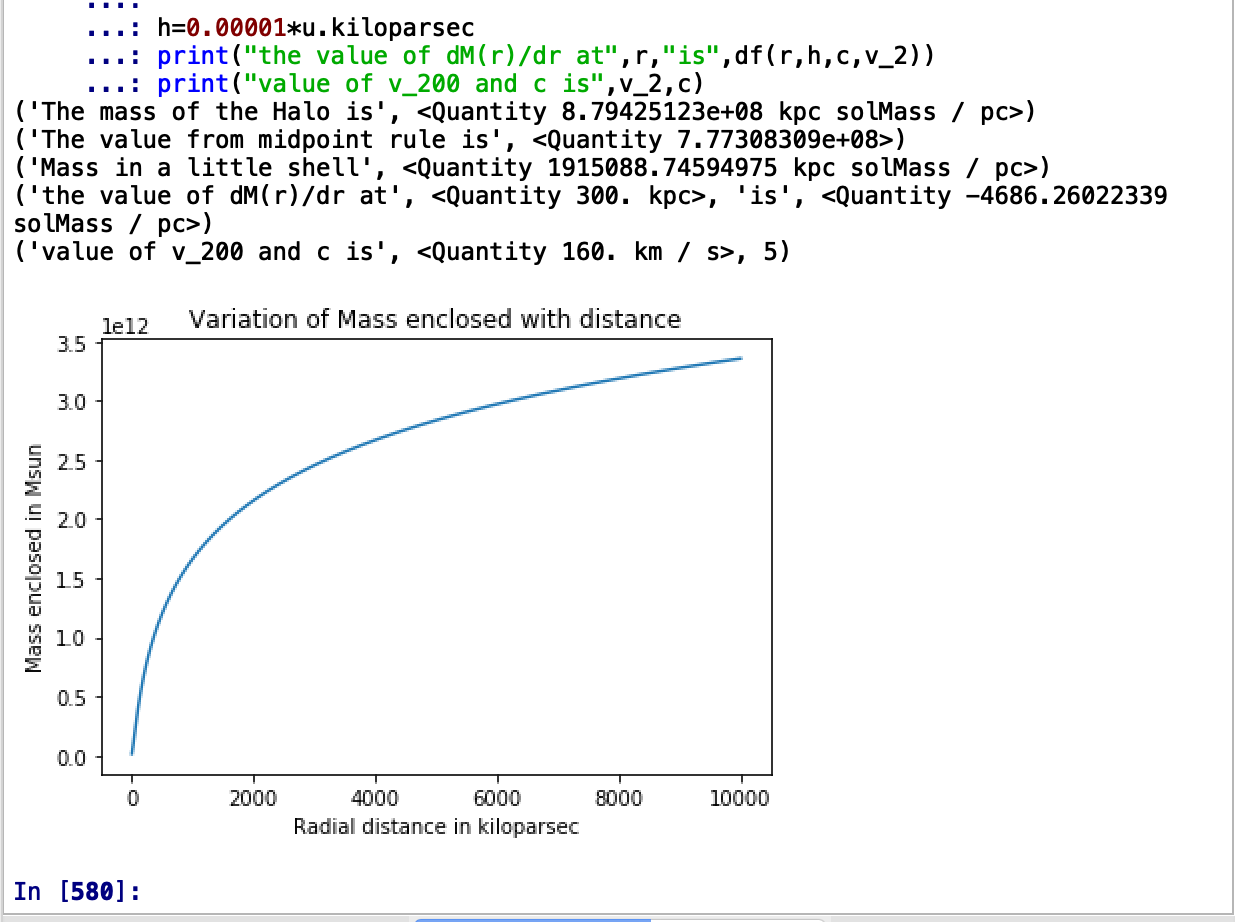
\includegraphics[scale=0.25]{Images/5}
        \end{center}
\columnbreak
	\begin{center}
       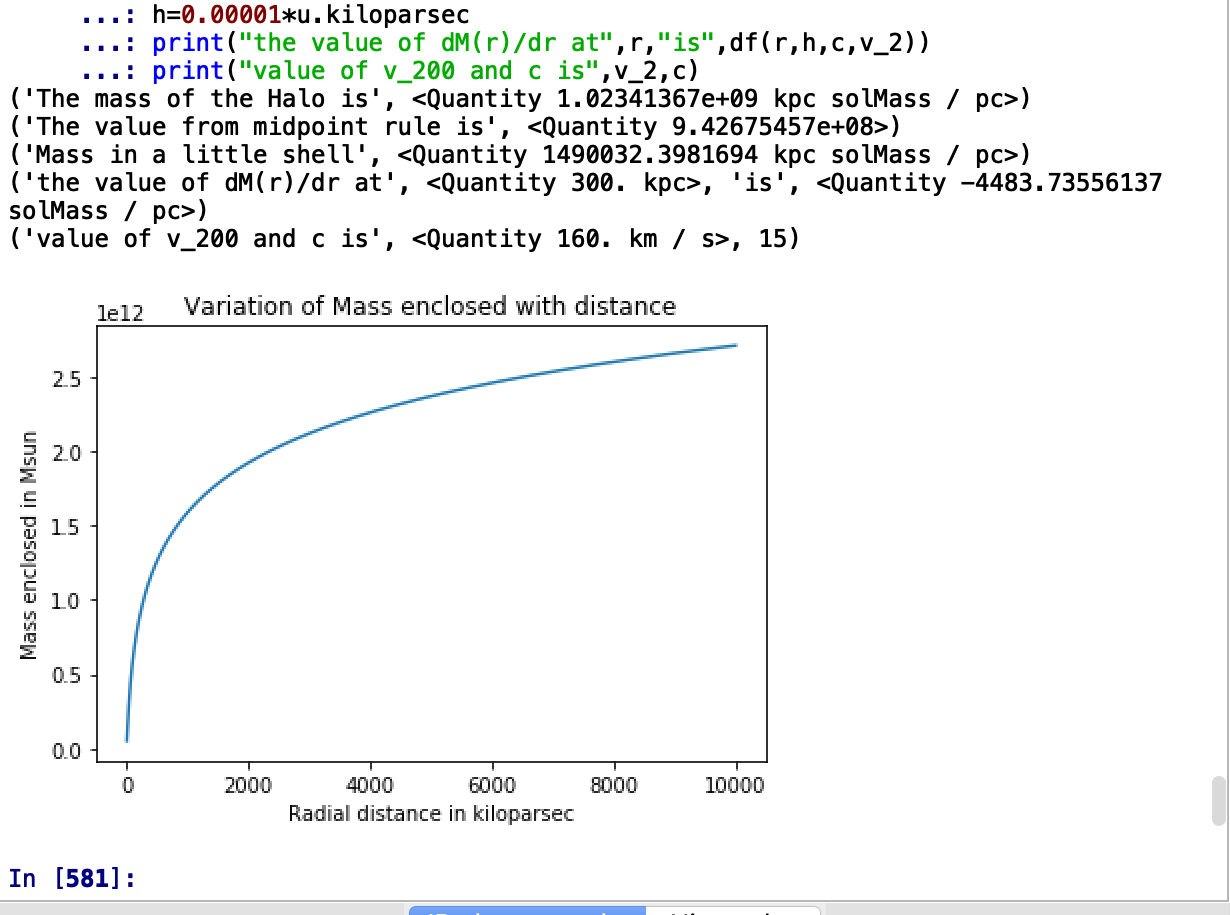
\includegraphics[scale=0.25]{Images/15}
       \end{center}
\end{multicols}
\end{center}

\begin{center}
\begin{multicols}{2}
	\begin{center}
        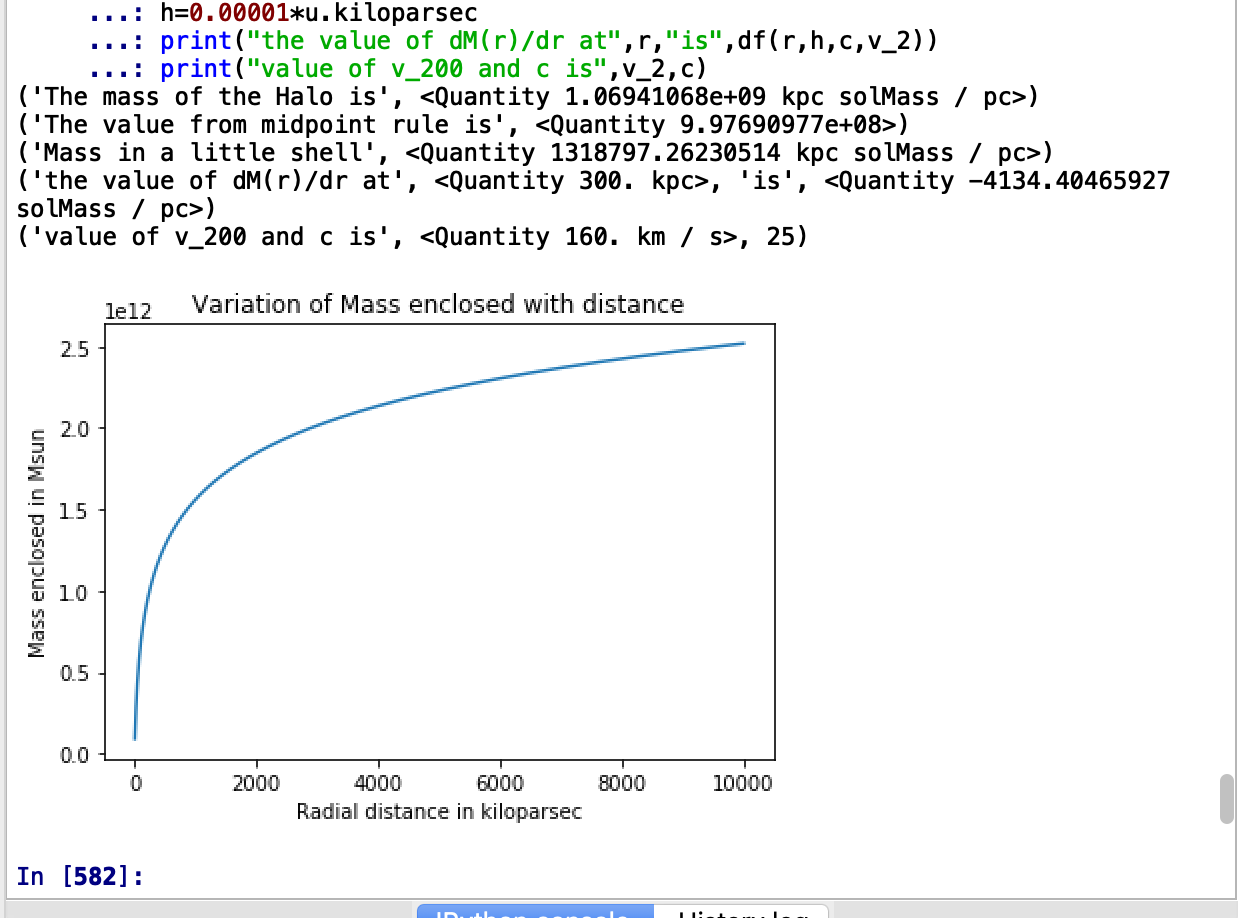
\includegraphics[scale=0.25]{Images/25}
        \end{center}
\columnbreak
	\begin{center}
       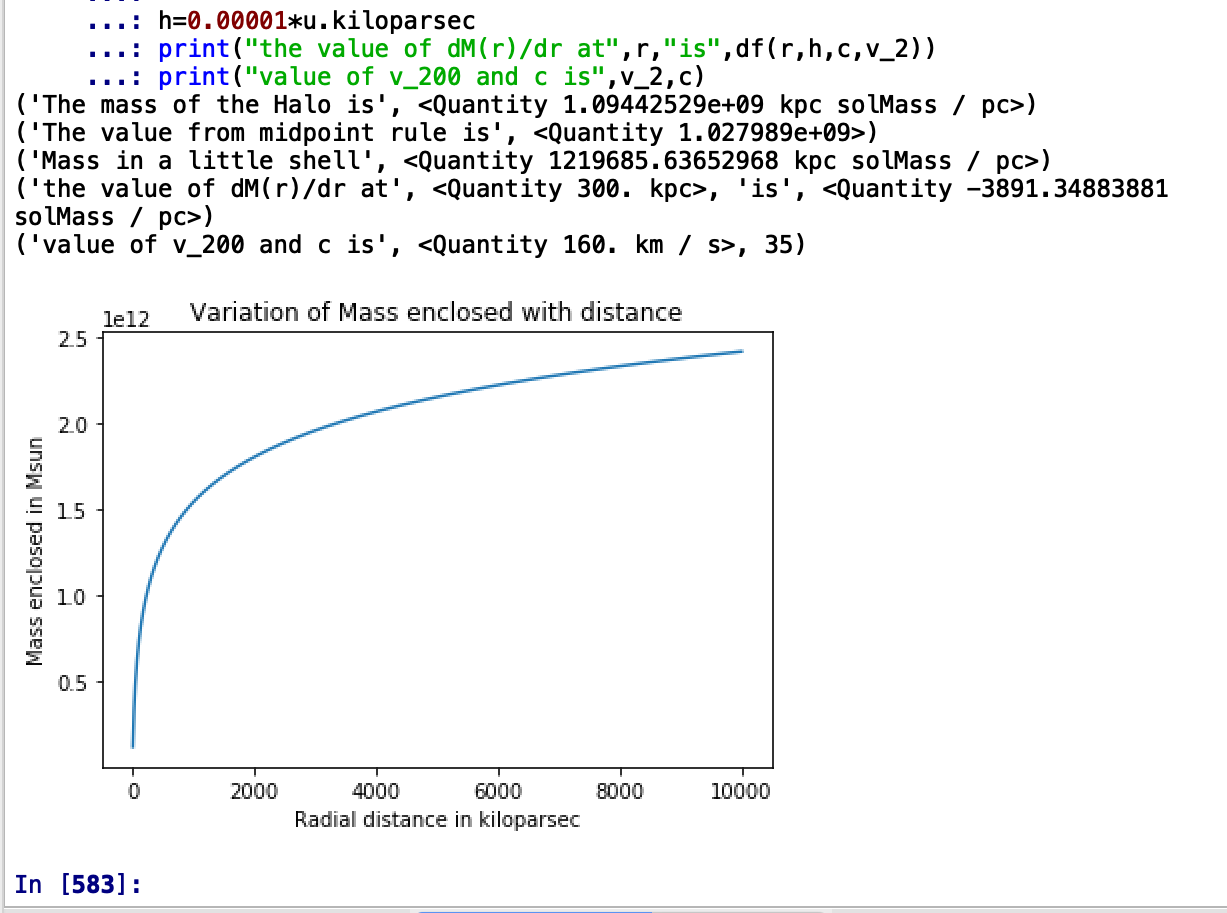
\includegraphics[scale=0.25]{Images/35}
       \end{center}
\end{multicols}
\end{center}


\emph{\small{These figures show output when I kept v200 fixed to 160 and changed c.}}
\vspace{0.5em}

As I increased c while keeping V200 constant, everything increased (dM(r)/dr becomes lesser negative).
\vspace{1.5em}

\textbf{Problem 3}\vspace{1.5em}

In this problem I have made a matrix class in which I have defined eight instances. \vspace{0.2em}

\begin{itemize}

\item{\textbf{init}}\vspace{0.2em} It has self and the matrix array as the argument. Here I defined 3 instance attributes, self.g gives back the array and helps me handle the array in a better way.
\item{\textbf{add(self,other)}}\vspace{0.2em} It takes self and the other(matrix) as the argument. I have included a check to see if addition is possible
\item{\textbf{mult(self,other)}}\vspace{0.2em} It takes self and the other(matrix) as the argument. I have included a check to see if multiplication is possible
\item{\textbf{tran(self)}}\vspace{0.2em}It takes self as argument and gives out Transpose as output.
\item{\textbf{trace(self)}}\vspace{0.2em}It takes self as argument and gives out Trace as output.
\item{\textbf{Det(self)}}\vspace{0.2em}It takes self as argument and gives out Determinant as output.

\begin{center}
\begin{multicols}{2}
	\begin{center}
        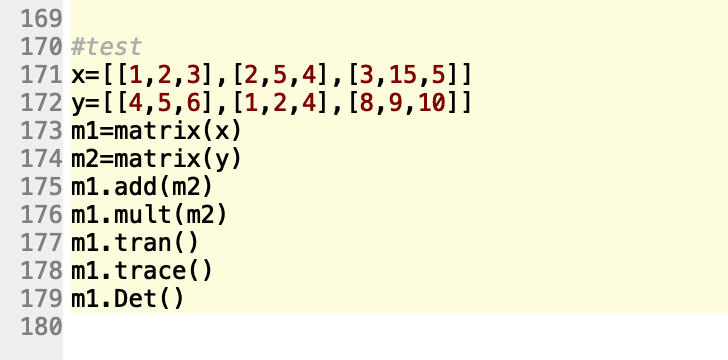
\includegraphics[scale=0.5]{Images/pb2test}
        \end{center}
\columnbreak
	\begin{center}
       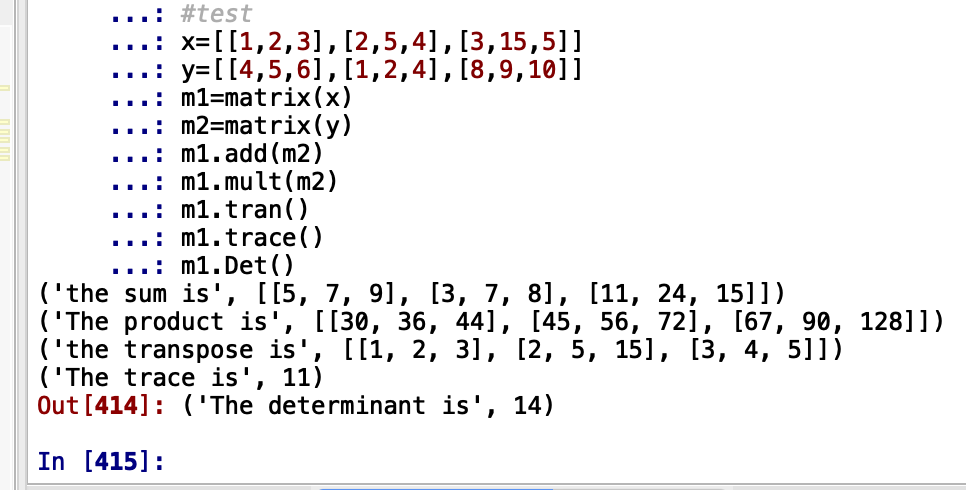
\includegraphics[scale=0.37]{Images/pb2testp}
       \end{center}
\end{multicols}
\end{center}
\emph{\small{Testing the instances using a matrix(the figure on the left), the results of the test(the figure on the right)}}
\item{\textbf{LU(self)}}\vspace{0.2em}Takes in self as argument and gives out lower and upper triangular matrix (in that order). In the figure I multiplies the L and U matrix and got the original matrix back.

\begin{center}
	 \emph{\small{Testing the LU Instance using a matrix}}
	 
	 \vspace{0.2em}

        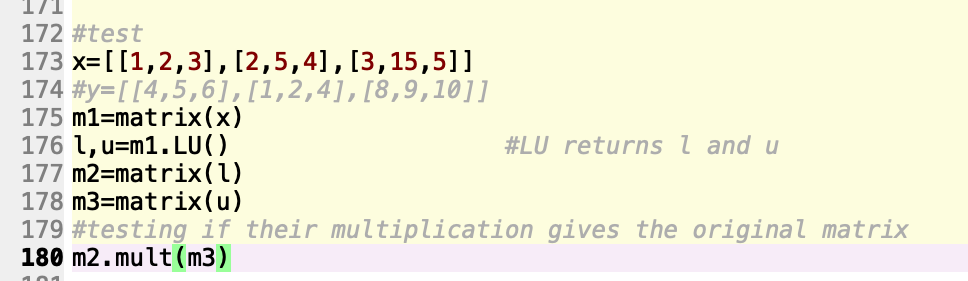
\includegraphics[scale=0.4]{Images/LUtest}
        
        
      
        
        \vspace{0.2em}
        
       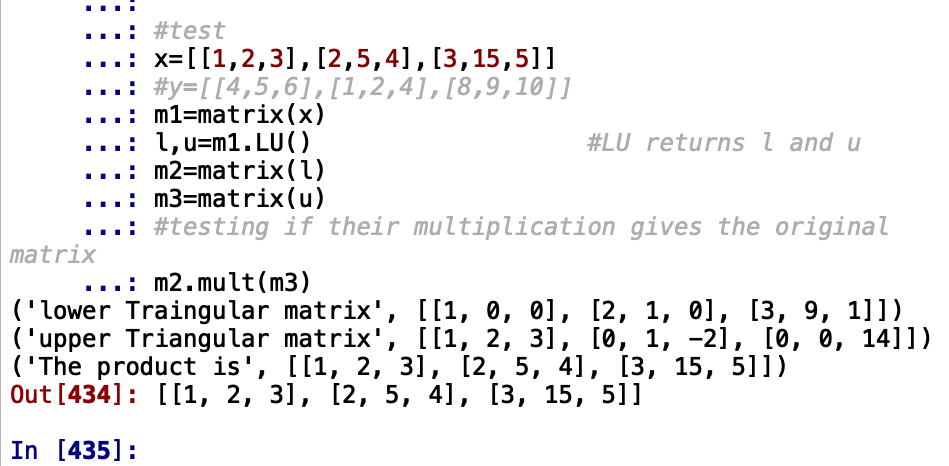
\includegraphics[scale=0.4]{Images/LUP}
       
       \vspace{0.2em}
       
       \emph{\small{Results of the test}}
\end{center}

\item{\textbf{Inv(self)}}\vspace{0.2em}Takes self as the argument and gives out the inverse.

\begin{center}
	
	 
	

        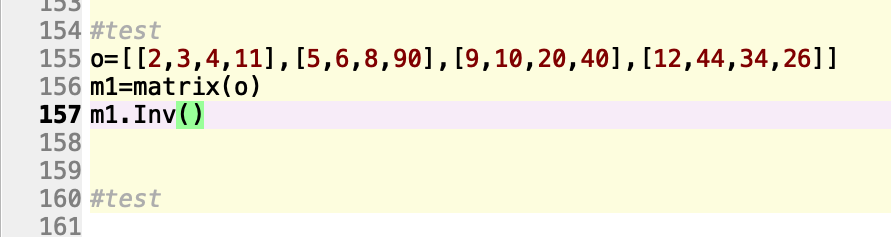
\includegraphics[scale=0.4]{Images/invtest}
        
         \vspace{0.2em}
       \emph{\small{Testing the Inv Instance using a matrix}}
        
        \vspace{0.2em}
        
       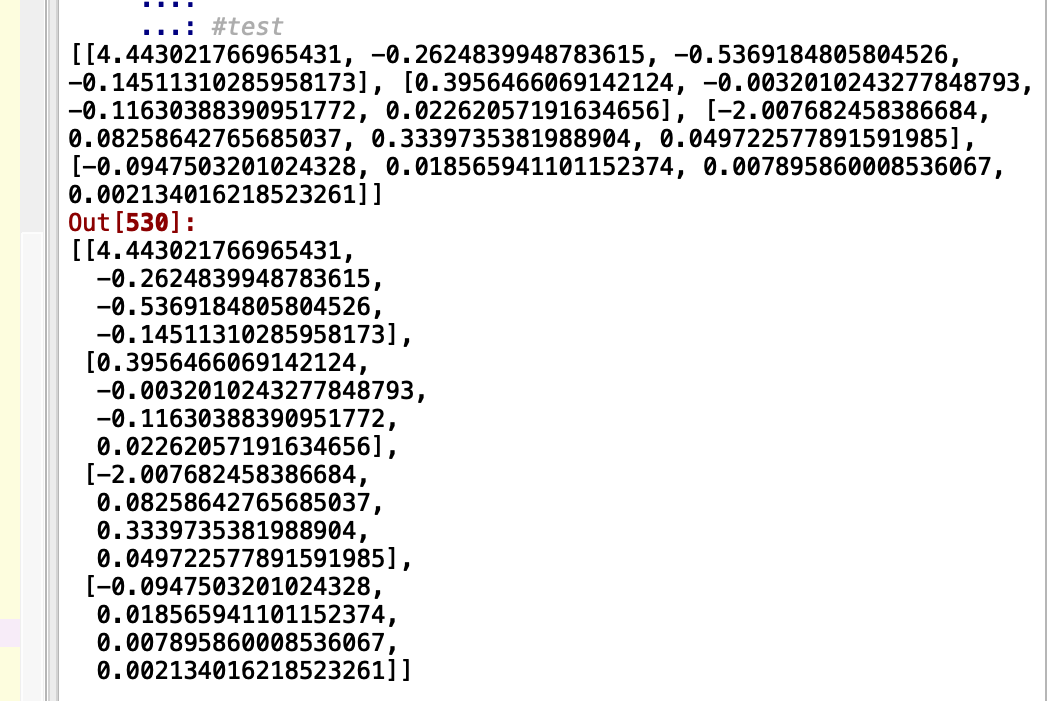
\includegraphics[scale=0.3]{Images/invtestp}
       
       \vspace{0.2em}
       
       \emph{\small{Results of the test}}
       \end{center}

\vspace{0.2em}

\end{itemize}
\emph{\small{I multiplied the result of the inverse with the original and got the identity matrix}}
\begin{center}
        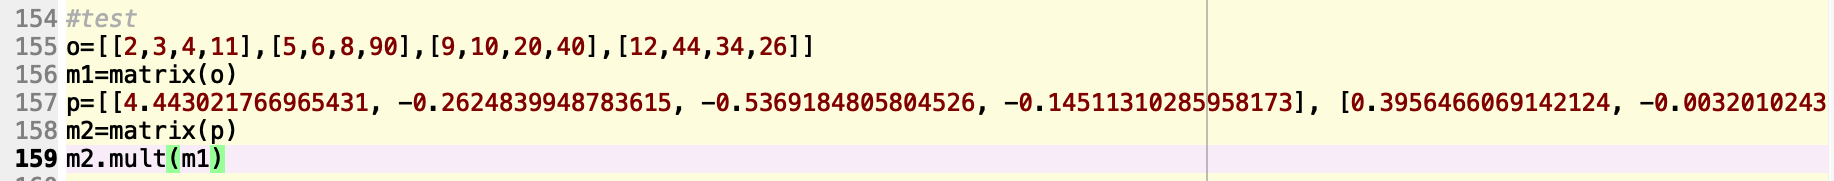
\includegraphics[scale=0.5]{Images/1}

       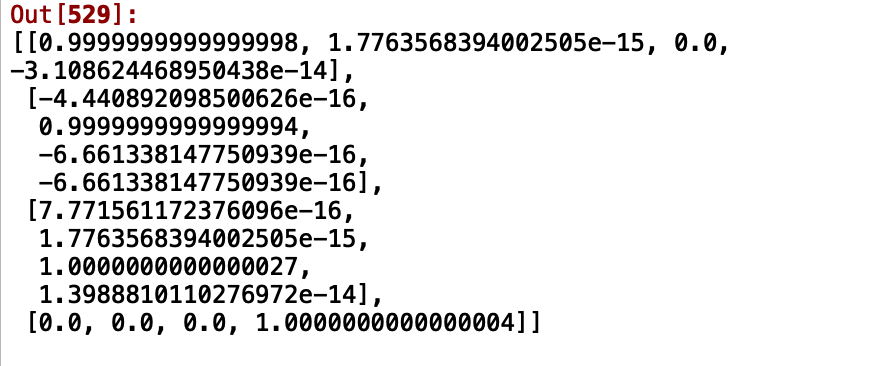
\includegraphics[scale=0.37]{Images/1p}
\end{center}

\vspace{0.2em}
\end{document}
